\documentclass[a4paper,12pt,twoside]{memoir}

% Castellano
\usepackage[spanish,es-tabla]{babel}
\selectlanguage{spanish}
\usepackage[utf8]{inputenc}
\usepackage[T1]{fontenc}
\usepackage{lmodern} % Scalable font
\usepackage{microtype}
\usepackage{placeins}

\RequirePackage{booktabs}
\RequirePackage[table]{xcolor}
\RequirePackage{xtab}
\RequirePackage{multirow}

% Links
\usepackage[colorlinks]{hyperref}
\hypersetup{
	allcolors = {red}
}

% Ecuaciones
\usepackage{amsmath}

% Rutas de fichero / paquete
\newcommand{\ruta}[1]{{\sffamily #1}}

% Párrafos
\nonzeroparskip


% Imagenes
\usepackage{graphicx}
\newcommand{\imagen}[2]{
	\begin{figure}[!h]
		\centering
		\includegraphics[width=0.9\textwidth]{#1}
		\caption{#2}\label{fig:#1}
	\end{figure}
	\FloatBarrier
}

\newcommand{\imagenflotante}[2]{
	\begin{figure}%[!h]
		\centering
		\includegraphics[width=0.9\textwidth]{#1}
		\caption{#2}\label{fig:#1}
	\end{figure}
}



% El comando \figura nos permite insertar figuras comodamente, y utilizando
% siempre el mismo formato. Los parametros son:
% 1 -> Porcentaje del ancho de página que ocupará la figura (de 0 a 1)
% 2 --> Fichero de la imagen
% 3 --> Texto a pie de imagen
% 4 --> Etiqueta (label) para referencias
% 5 --> Opciones que queramos pasarle al \includegraphics
% 6 --> Opciones de posicionamiento a pasarle a \begin{figure}
\newcommand{\figuraConPosicion}[6]{%
  \setlength{\anchoFloat}{#1\textwidth}%
  \addtolength{\anchoFloat}{-4\fboxsep}%
  \setlength{\anchoFigura}{\anchoFloat}%
  \begin{figure}[#6]
    \begin{center}%
      \Ovalbox{%
        \begin{minipage}{\anchoFloat}%
          \begin{center}%
            \includegraphics[width=\anchoFigura,#5]{#2}%
            \caption{#3}%
            \label{#4}%
          \end{center}%
        \end{minipage}
      }%
    \end{center}%
  \end{figure}%
}

%
% Comando para incluir imágenes en formato apaisado (sin marco).
\newcommand{\figuraApaisadaSinMarco}[5]{%
  \begin{figure}%
    \begin{center}%
    \includegraphics[angle=90,height=#1\textheight,#5]{#2}%
    \caption{#3}%
    \label{#4}%
    \end{center}%
  \end{figure}%
}
% Para las tablas
\newcommand{\otoprule}{\midrule [\heavyrulewidth]}
%
% Nuevo comando para tablas pequeñas (menos de una página).
\newcommand{\tablaSmall}[5]{%
 \begin{table}
  \begin{center}
   \rowcolors {2}{gray!35}{}
   \begin{tabular}{#2}
    \toprule
    #4
    \otoprule
    #5
    \bottomrule
   \end{tabular}
   \caption{#1}
   \label{tabla:#3}
  \end{center}
 \end{table}
}

%
% Nuevo comando para tablas pequeñas (menos de una página).
\newcommand{\tablaSmallSinColores}[5]{%
 \begin{table}[H]
  \begin{center}
   \begin{tabular}{#2}
    \toprule
    #4
    \otoprule
    #5
    \bottomrule
   \end{tabular}
   \caption{#1}
   \label{tabla:#3}
  \end{center}
 \end{table}
}

\newcommand{\tablaApaisadaSmall}[5]{%
\begin{landscape}
  \begin{table}
   \begin{center}
    \rowcolors {2}{gray!35}{}
    \begin{tabular}{#2}
     \toprule
     #4
     \otoprule
     #5
     \bottomrule
    \end{tabular}
    \caption{#1}
    \label{tabla:#3}
   \end{center}
  \end{table}
\end{landscape}
}

%
% Nuevo comando para tablas grandes con cabecera y filas alternas coloreadas en gris.
\newcommand{\tabla}[6]{%
  \begin{center}
    \tablefirsthead{
      \toprule
      #5
      \otoprule
    }
    \tablehead{
      \multicolumn{#3}{l}{\small\sl continúa desde la página anterior}\\
      \toprule
      #5
      \otoprule
    }
    \tabletail{
      \hline
      \multicolumn{#3}{r}{\small\sl continúa en la página siguiente}\\
    }
    \tablelasttail{
      \hline
    }
    \bottomcaption{#1}
    \rowcolors {2}{gray!35}{}
    \begin{xtabular}{#2}
      #6
      \bottomrule
    \end{xtabular}
    \label{tabla:#4}
  \end{center}
}

%
% Nuevo comando para tablas grandes con cabecera.
\newcommand{\tablaSinColores}[6]{%
  \begin{center}
    \tablefirsthead{
      \toprule
      #5
      \otoprule
    }
    \tablehead{
      \multicolumn{#3}{l}{\small\sl continúa desde la página anterior}\\
      \toprule
      #5
      \otoprule
    }
    \tabletail{
      \hline
      \multicolumn{#3}{r}{\small\sl continúa en la página siguiente}\\
    }
    \tablelasttail{
      \hline
    }
    \bottomcaption{#1}
    \begin{xtabular}{#2}
      #6
      \bottomrule
    \end{xtabular}
    \label{tabla:#4}
  \end{center}
}

%
% Nuevo comando para tablas grandes sin cabecera.
\newcommand{\tablaSinCabecera}[5]{%
  \begin{center}
    \tablefirsthead{
      \toprule
    }
    \tablehead{
      \multicolumn{#3}{l}{\small\sl continúa desde la página anterior}\\
      \hline
    }
    \tabletail{
      \hline
      \multicolumn{#3}{r}{\small\sl continúa en la página siguiente}\\
    }
    \tablelasttail{
      \hline
    }
    \bottomcaption{#1}
  \begin{xtabular}{#2}
    #5
   \bottomrule
  \end{xtabular}
  \label{tabla:#4}
  \end{center}
}



\definecolor{cgoLight}{HTML}{EEEEEE}
\definecolor{cgoExtralight}{HTML}{FFFFFF}

%
% Nuevo comando para tablas grandes sin cabecera.
\newcommand{\tablaSinCabeceraConBandas}[5]{%
  \begin{center}
    \tablefirsthead{
      \toprule
    }
    \tablehead{
      \multicolumn{#3}{l}{\small\sl continúa desde la página anterior}\\
      \hline
    }
    \tabletail{
      \hline
      \multicolumn{#3}{r}{\small\sl continúa en la página siguiente}\\
    }
    \tablelasttail{
      \hline
    }
    \bottomcaption{#1}
    \rowcolors[]{1}{cgoExtralight}{cgoLight}

  \begin{xtabular}{#2}
    #5
   \bottomrule
  \end{xtabular}
  \label{tabla:#4}
  \end{center}
}


















\graphicspath{ {./img/} }

% Capítulos
\chapterstyle{bianchi}
\newcommand{\capitulo}[2]{
	\setcounter{chapter}{#1}
	\setcounter{section}{0}
	\chapter*{#2}
	\addcontentsline{toc}{chapter}{#2}
	\markboth{#2}{#2}
}

% Apéndices
\renewcommand{\appendixname}{Apéndice}
\renewcommand*\cftappendixname{\appendixname}

\newcommand{\apendice}[1]{
	%\renewcommand{\thechapter}{A}
	\chapter{#1}
}

\renewcommand*\cftappendixname{\appendixname\ }

% Formato de portada
\makeatletter
\usepackage{xcolor}
\newcommand{\tutor}[1]{\def\@tutor{#1}}
\newcommand{\course}[1]{\def\@course{#1}}
\definecolor{cpardoBox}{HTML}{E6E6FF}
\def\maketitle{
  \null
  \thispagestyle{empty}
  % Cabecera ----------------
\noindent
\includegraphics[width=\textwidth]{cabecera}\vspace{1cm}%
  \vfill
  % Título proyecto y escudo informática ----------------
  \colorbox{cpardoBox}{%
    \begin{minipage}{.8\textwidth}
      \vspace{.5cm}\Large
      \begin{center}
      \textbf{TFG del Grado en Ingeniería Informática}\vspace{.6cm}\\
      \textbf{\LARGE\@title{}}
      \end{center}
      \vspace{.2cm}
    \end{minipage}

  }%
  \hfill\begin{minipage}{.20\textwidth}
    
\includegraphics[width=\textwidth]{escudoInfor}
  \end{minipage}
  \vfill
  % Datos de alumno, curso y tutores ------------------
  \begin{center}%
  {%
    \noindent\LARGE
    Presentado por \@author{}\\ 
    en Universidad de Burgos --- \@date{}\\
    Tutor: \@tutor{}\\
  }%
  \end{center}%
  \null
  \cleardoublepage
  }
\makeatother

\newcommand{\nombre}{Nombre del alumno} %%% cambio de comando

% Datos de portada
\title{título del TFG}
\author{\nombre}
\tutor{nombre tutor}
\date{\today}

\begin{document}

\maketitle


\newpage\null\thispagestyle{empty}\newpage


%%%%%%%%%%%%%%%%%%%%%%%%%%%%%%%%%%%%%%%%%%%%%%%%%%%%%%%%%%%%%%%%%%%%%%%%%%%%%%%%%%%%%%%%
\thispagestyle{empty}


\noindent
\includegraphics[width=\textwidth]{cabecera}\vspace{1cm}

\noindent D. nombre tutor, profesor del departamento de nombre departamento, área de nombre área.

\noindent Expone:

\noindent Que el alumno D. \nombre, con DNI dni, ha realizado el Trabajo final de Grado en Ingeniería Informática titulado título de TFG. 

\noindent Y que dicho trabajo ha sido realizado por el alumno bajo la dirección del que suscribe, en virtud de lo cual se autoriza su presentación y defensa.

\begin{center} %\large
En Burgos, {\large \today}
\end{center}

\vfill\vfill\vfill

% Author and supervisor
\begin{minipage}{0.45\textwidth}
\begin{flushleft} %\large
Vº. Bº. del Tutor:\\[2cm]
D. nombre tutor
\end{flushleft}
\end{minipage}
\hfill
\begin{minipage}{0.45\textwidth}
\begin{flushleft} %\large
Vº. Bº. del co-tutor:\\[2cm]
D. nombre co-tutor
\end{flushleft}
\end{minipage}
\hfill

\vfill

% para casos con solo un tutor comentar lo anterior
% y descomentar lo siguiente
%Vº. Bº. del Tutor:\\[2cm]
%D. nombre tutor


\newpage\null\thispagestyle{empty}\newpage




\frontmatter

% Abstract en castellano
\renewcommand*\abstractname{Resumen}
\begin{abstract}
En este primer apartado se hace una \textbf{breve} presentación del tema que se aborda en el proyecto.
\end{abstract}

\renewcommand*\abstractname{Descriptores}
\begin{abstract}
Palabras separadas por comas que identifiquen el contenido del proyecto Ej: servidor web, buscador de vuelos, android \ldots
\end{abstract}

\clearpage

% Abstract en inglés
\renewcommand*\abstractname{Abstract}
\begin{abstract}
A \textbf{brief} presentation of the topic addressed in the project.
\end{abstract}

\renewcommand*\abstractname{Keywords}
\begin{abstract}
keywords separated by commas.
\end{abstract}

\clearpage

% Indices
\tableofcontents

\clearpage

\listoffigures

\clearpage

\listoftables
\clearpage

\mainmatter
\capitulo{1}{Introducción}

El control de calidad es un aspecto importante de los procesos de fabricación. Ha aumentado el nivel de competencia en el mercado de fabricación por lo que los fabricantes deben aumentar su tasa de producción manteniendo los límites de calidad para los productos.

Las piezas de aluminio tienen actualmente un alto interés tecnológico en diversos sectores industriales (como el del automóvil) debido, entre otras, a propiedades de interés, como:

\begin{itemize}
    \item Su ligereza.
    \item Su óptima conductividad térmica y eléctrica (un conductor de aluminio pesa sólo la mitad que un conductor de cobre equivalente).
    \item Su alto porcentaje de reciclabilidad.
\end{itemize}

No obstante, durante su creación se pueden crear pequeñas burbujas o poros que son indetectables por el ojo humano aun encontrándose en la superficie. Estas burbujas pueden hacer que la pieza se rompa durante su periodo de uso, pudiendo llegar a ser un problema crítico en el caso, por ejemplo, de las piezas de automóviles ya que están sometidas a una fatiga continua.

Hay una serie de exámenes no destructivos (\textit{nondestructive examination} - NDE) que son técnicas disponibles para producir imágenes bidimensionales y tridimensionales de un objeto tales como: imágenes de rayos-X, inspección ultrasónica, inspección de partículas magnéticas u otras.

Actualmente el análisis (inspección) de estas piezas se realiza de manera visual y subjetiva por parte de personal de la propia empresa. Los empleados examinan las imágenes de rayos-X y determinan la posición de los defectos en el caso de que haya. Este proceso de análisis presenta dos grandes desventajas: el cansancio y el cambio de criterio del operario, con el paso del tiempo. Además, cada operario tiene un criterio diferente de evaluación, dificultando un seguimiento objetivo de la calidad.

La finalidad del proyecto es la de aplicar un sistema de aprendizaje basado en una red neuronal, para la identificación de estos defectos en imágenes de rayos-X tomadas principalmente de partes automotrices (ruedas de aluminio y nudillos).

El objetivo final a largo plazo sería poder comprobar la validez de una metodología automatizada que permita reducir costes y hacer el proceso más robusto y objetivo.

\section{Estructura de la memoria}

Esta memoria incluye los siguientes apartados:

\begin{itemize}
    \item \textbf{Introducción:} Breve descripción del problema a resolver y la solución propuesta. Estructura de la memoria y listado de materiales adjuntos.
    \item \textbf{Objetivos del proyecto:} Exposición de los    objetivos generales, técnicos y personales del proyecto.
    \item \textbf{Conceptos teóricos:} Breve explicación de los conceptos teóricos necesarios para la comprensión y el desarrollo del proyecto.
    \item \textbf{Técnicas y herramientas:} Presentación de las técnicas metodológicas y las herramientas de desarrollo que se han utilizado para llevar a cabo el proyecto.
    \item \textbf{Aspectos relevantes del desarrollo:} Listado o exposición de los aspectos más importantes durante el desarrollo del proyecto.
    \item \textbf{Trabajos relacionados:} Breve resumen de los trabajos y proyectos vinculados con la detección de defectos en imágenes de rayos-X y el estado del arte del proyecto.
    \item \textbf{Conclusiones y líneas de trabajo futuras:} Conclusiones obtenidas al final del proyecto y exposición de posibles mejoras o líneas de trabajo futuro.
\end{itemize}

\section{Materiales adjuntos}

Anexos aportados junto a la memoria:

\begin{itemize}
    \item \textbf{Plan del proyecto software:} Planificación temporal y estudio de viabilidad económica y legal del proyecto.
    \item \textbf{Especificación de requisitos del software:} Objetivos generales, catálogo de requisitos del sistema y especificación de requisitos funcionales y no funcionales.
    \item \textbf{Especificación de diseño:} Diseño de datos, diseño procedimental y diseño arquitectónico.
    \item \textbf{Manual del programador:} Estructura de directorios, manual del programador, compilación, instalación ejecución y pruebas (aspectos relevantes del código fuente).
    \item \textbf{Manual de usuario:} Requisitos de usuarios, instalación, manual de usuario.
\end{itemize}

Repositorio del proyecto accesible a través de internet \url{https://github.com/nuf1001/XRayDetector/} \cite{XRayDetector:repositorio}.
\capitulo{2}{Objetivos del proyecto}

Este apartado explica de forma precisa y concisa cuales son los objetivos que se persiguen con la realización del proyecto. Se puede distinguir entre los objetivos marcados por los requisitos del software a construir y los objetivos de carácter técnico que plantea a la hora de llevar a la práctica el proyecto.

\capitulo{3}{Conceptos teóricos}

En aquellos proyectos que necesiten para su comprensión y desarrollo de unos conceptos teóricos de una determinada materia o de un determinado dominio de conocimiento, debe existir un apartado que sintetice dichos conceptos.

Algunos conceptos teóricos de \LaTeX \footnote{Créditos a los proyectos de Álvaro López Cantero: Configurador de Presupuestos y Roberto Izquierdo Amo: PLQuiz}.

\section{Secciones}

Las secciones se incluyen con el comando section.

\subsection{Subsecciones}

Además de secciones tenemos subsecciones.

\subsubsection{Subsubsecciones}

Y subsecciones. 


\section{Referencias}

Las referencias se incluyen en el texto usando cite \cite{wiki:latex}. Para citar webs, artículos o libros \cite{koza92}.


\section{Imágenes}

Se pueden incluir imágenes con los comandos standard de \LaTeX, pero esta plantilla dispone de comandos propios como por ejemplo el siguiente:

\imagen{escudoInfor}{Autómata para una expresión vacía}



\section{Listas de items}

Existen tres posibilidades:

\begin{itemize}
	\item primer item.
	\item segundo item.
\end{itemize}

\begin{enumerate}
	\item primer item.
	\item segundo item.
\end{enumerate}

\begin{description}
	\item[Primer item] más información sobre el primer item.
	\item[Segundo item] más información sobre el segundo item.
\end{description}
	
\begin{itemize}
\item 
\end{itemize}

\section{Tablas}

Igualmente se pueden usar los comandos específicos de \LaTeX o bien usar alguno de los comandos de la plantilla.

\tablaSmall{Herramientas y tecnologías utilizadas en cada parte del proyecto}{l c c c c}{herramientasportipodeuso}
{ \multicolumn{1}{l}{Herramientas} & App AngularJS & API REST & BD & Memoria \\}{ 
HTML5 & X & & &\\
CSS3 & X & & &\\
BOOTSTRAP & X & & &\\
JavaScript & X & & &\\
AngularJS & X & & &\\
Bower & X & & &\\
PHP & & X & &\\
Karma + Jasmine & X & & &\\
Slim framework & & X & &\\
Idiorm & & X & &\\
Composer & & X & &\\
JSON & X & X & &\\
PhpStorm & X & X & &\\
MySQL & & & X &\\
PhpMyAdmin & & & X &\\
Git + BitBucket & X & X & X & X\\
Mik\TeX{} & & & & X\\
\TeX{}Maker & & & & X\\
Astah & & & & X\\
Balsamiq Mockups & X & & &\\
VersionOne & X & X & X & X\\
} 

\capitulo{4}{Técnicas y herramientas}

Esta parte de la memoria tiene como objetivo presentar las técnicas metodológicas y las herramientas de desarrollo que se han utilizado para llevar a cabo el proyecto. Si se han estudiado diferentes alternativas de metodologías, herramientas, bibliotecas se puede hacer un resumen de los aspectos más destacados de cada alternativa, incluyendo comparativas entre las distintas opciones y una justificación de las elecciones realizadas. 
No se pretende que este apartado se convierta en un capítulo de un libro dedicado a cada una de las alternativas, sino comentar los aspectos más destacados de cada opción, con un repaso somero a los fundamentos esenciales y referencias bibliográficas para que el lector pueda ampliar su conocimiento sobre el tema.



\capitulo{5}{Aspectos relevantes del desarrollo del proyecto}

\section{Introducción}

En este apartado explicamos el entrenamiento (\nameref{SectionEntrenamiento}) de nuestra red y las salidas que obtenemos. Comparamos los dos últimos modelos para ver cuál de ellos lo utilizamos para la aplicación de escritorio (\nameref{SectionComparacion}) y realizamos algunas pruebas al modelo seleccionado (\nameref{SectionPruebasModelo}).

También veremos las gráficas con los valores obtenidos tras el entrenamiento (\nameref{SectionGraficas}).

\subsection{Vocabulario}

Las palabras relacionadas con este apartado son:

\begin{itemize}
    \item \textbf{\textit{Steps}:} Un \textit{step} es un paso en el entrenamiento de la red neuronal. Tras finalizar un \textit{step} los datos de salida se utilizan para entrenar el siguiente.
    \item \textbf{\textit{Epochs}:} Son las etapas de nuestra red neuronal, por cada \textit{epoch} que se ejecuta se crea un modelo válido para  predecir defectos en nuevas imágenes. Una \textit{epoch} está formada por varios \textit{steps}, puedes asignar el número que mejor te convenga, en nuestro proyecto se ejecutan 500 \textit{steps} por \textit{epoch}.
    \item \textbf{\textit{Bounding Box}:} Cuadro delimitado donde se encuentran los defectos. Son cuatro valores que representan las coordenadas (\textit{x},\textit{y}) de las esquinas superior izquierda e inferior derecha del cuadro delimitador.
    \item \textbf{AP (\textit{Average Precision}):} Este término esta explicado en \ref{SectionAP}, el máximo que se puede obtener es de 1.
\end{itemize}

\section{Entrenamiento\label{SectionEntrenamiento}}

Para el entrenamiento de esta red se divide en tres etapas:

\begin{itemize}
    \item \textbf{Primera etapa:} Son 40 \textit{epochs} entrenando la cabecera de la red.
    \item \textbf{Segunda etapa:} Son 80 \textit{epochs} entrenando de la etapa 4 y superiores de la red.
    \item \textbf{Tercera etapa:} Son 40 \textit{epochs} entrenando todas las capas de la red.
\end{itemize}

\begin{figure}[h]
    \centering
    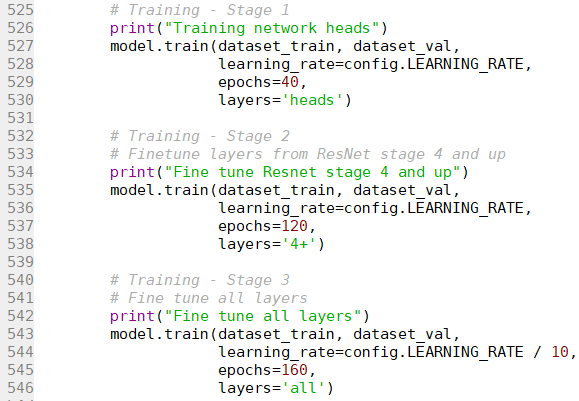
\includegraphics[width=0.63\textwidth]{codentrenamiento}
    \caption{Etapas de entrenamiento del código}
    \label{codentrenamiento}
\end{figure}

Esto es sólo una posible forma de entrenar la red (es la recomendada por Max Ferguson en su repositorio \cite{metal-defect-detection:repositorio}), hay más formas de entrenar la red, los parámetros para seleccionar que capas quieres entrenar son:

\begin{itemize}
    \item \textbf{heads:} Entrena la RPN, los clasificadores y los cabezales de máscara de la red.
    \item \textbf{all:} Todas las capas.
    \item \textbf{3+:} Entrena Resnet etapa 3 y superior.
    \item \textbf{4+:} Entrena Resnet etapa 4 y superior.
    \item \textbf{5+:} Entrena Resnet etapa 5 y superior.
    \item Una expresión regular para unir los nombres de las capas para entrenar.
\end{itemize}

Estas etapas están explicadas en \ref{resnetLabel}.

\begin{figure}[h]
	\centering
	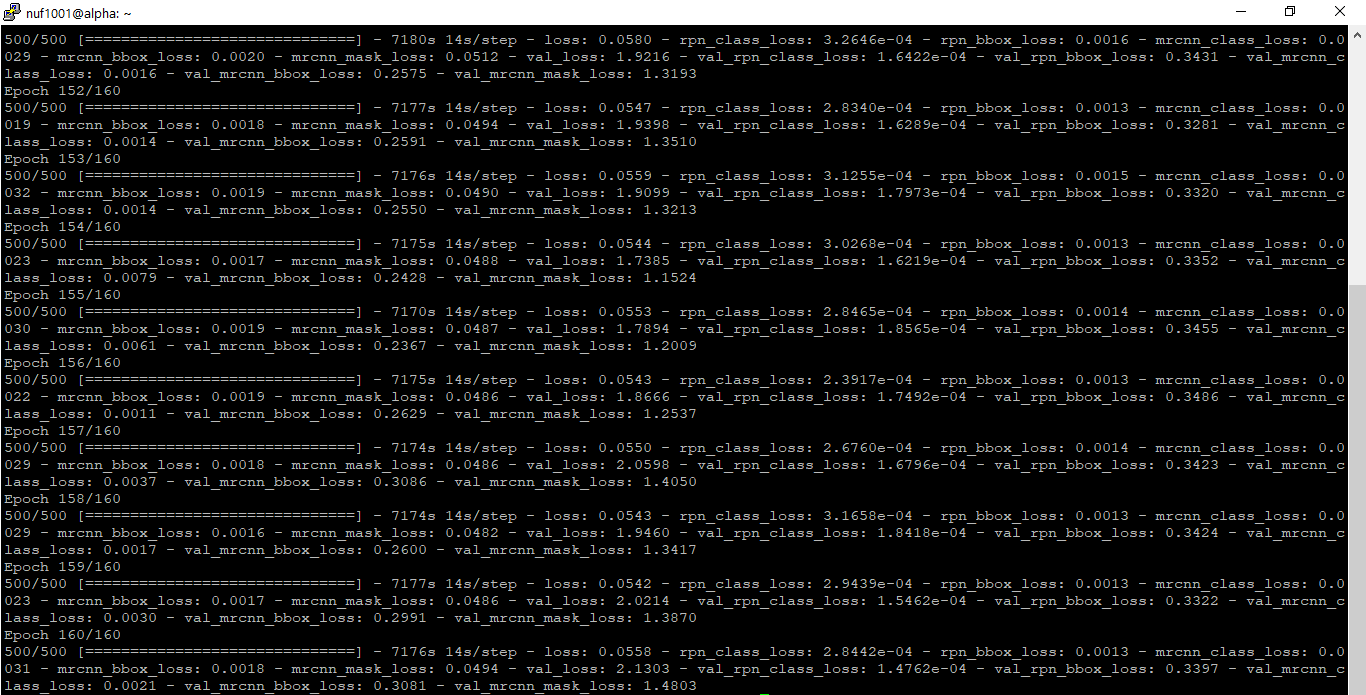
\includegraphics[width=1.3\textwidth]{entrenamiento160}
	\caption{Últimas \textit{epochs} del entrenamiento}
	\label{entrenamiento160}
\end{figure}

Se guarda un modelo por cada \textit{epoch}, es decir, al final del entrenamiento tendremos 160 modelos con 500 \textit{steps} por cada una, 80.000 \textit{steps} en total.

En la figura \ref{entrenamiento160} podemos ver la salida por pantalla del final del entrenamiento, las últimas 10 \textit{epochs} que se han realizado. Se va ha hacer incapié en las dos últimas \textit{epochs} la 159 y la 160 para saber cuál de los dos modelos es el mejor entrenado.

Los 5 \textit{losses} que vemos en la figura \ref{entrenamiento160} representan\label{losses}:

\begin{itemize}
    \item \textbf{rpn\_class\_loss:} Qué tan bien la red de propuestas de la región separa el fondo con los objetos, es decir, qué tan bien se diferencia el fondo (\textit{background} - BG) de los posibles defectos.
    \item \textbf{rpn\_bbox\_loss:} Qué tan bien los RPN localizan objetos.
    \item \textbf{mrcnn\_bbox\_loss:} Qué tan bien \textit{Mask RCNN} localiza objetos.
    \item \textbf{mrcnn\_class\_loss:} Qué tan bien \textit{Mask RCNN} reconoce cada clase de objeto.
    \item \textbf{mrcnn\_mask\_loss:} Qué tan bien \textit{Mask RCNN} segmenta los objetos.
\end{itemize}

Eso hace una mayor pérdida:

\begin{itemize}
    \item \textbf{\textit{loss}:} Una combinación de todos los \textit{losses} anteriores.
\end{itemize}

Todos estos \textit{losses} se calculan en el conjunto de datos de entrenamiento. Y los \textit{losses} para el conjunto de datos de validación son las que comienzan con ``val''.

\newpage

\subsection{Comparación modelos 159 y 160\label{SectionComparacion}}

\imagen{evaluate159_20}{Evaluación con el modelo número 159\label{evaluate159}}

\imagen{evaluate160_20}{Evaluación con el modelo número 160\label{evaluate160}}

Si comparamos los datos de la \textit{epoch} 160 y 159 que aparecen en las figuras \ref{entrenamiento160}, \ref{evaluate159} y \ref{evaluate160} vemos que la penúltima tiene mejores datos, es decir, el modelo 159 tiene un \textit{loss} menor que el modelo 160, ver en la tabla \ref{comparacionepochs}.

Como vemos en la tabla \ref{comparacionepochs} los datos los \textit{losses} de la \textit{epoch} 159 son mejores que los de la 160, pero vamos a hacer algunas pruebas para corroborarlo.

La diferencia de la mAP \cite{AP} que se observa en las figuras \ref{evaluate159} y \ref{evaluate160} no es muy grande, hay ocasiones en las que la evaluación del modelo 160 ha sido mejor que el del 159, pero predominan las pruebas con mejor AP en el modelo 159.

\newpage

\begin{table}[h]
	\begin{center}
		\begin{tabular}{l | c c c}
			Tipo de datos & \textit{Epoch} 159 & Comparación & \textit{Epoch} 160\\ \hline
			val\_loss & 2.0214 & < & 2.1303\\
			val\_rpn\_class\_loss & 1.5462e-04 & < & 1.4762e-04\\
			val\_rpn\_bbox\_loss & 0.3322 & < & 0.3397\\
			val\_mrcnn\_class\_loss & 0.0030 & > & 0.0021\\
			val\_mrcnn\_bbox\_loss & 0.2991 & < & 0.3081\\
			val\_mrcnn\_mask\_loss & 1.3870 & < & 1.4803\\
			mAP & 0.8583 & > & 0.8283\\
		\end{tabular}
		\caption{Comparación de las dos últimas \textit{epochs}}
		\label{comparacionepochs}
	\end{center}
\end{table}


\textbf{Imagen C0001\_0018:}

\imagen{img_C0001_0018_159}{Imagen C0001\_0018 con los \textit{Bounding Box} del modelo 159\label{img_C0001_0018_159}}

\imagen{tabla_C0001_0018_159}{Cuadrícula de la imagen C0001\_0018 de objetos de verdad y sus predicciones del modelo 159\label{tabla_C0001_0018_159}}

\imagen{img_C0001_0018_160}{Imagen C0001\_0018 con los \textit{Bounding Box} del modelo 160\label{img_C0001_0018_160}}

\imagen{tabla_C0001_0018_160}{Cuadrícula de la imagen C0001\_0018 de objetos de verdad y sus predicciones del modelo 160\label{tabla_C0001_0018_160}}

Las figuras \ref{img_C0001_0018_159} y \ref{img_C0001_0018_160} representa la imagen C0001\_0018 con los defectos detectados por los modelos 159 y 160 respectivamente. Las figuras \ref{tabla_C0001_0018_159} y \ref{tabla_C0001_0018_160} son las cuadriculas de los \textit{ground truth} y las predicciones hechas por los modelos entrenados. Las columnas representan los defectos reales que tiene la imagen y las filas los defectos detectados por el modelo, en este caso había tres defectos y los dos modelos han detectado los tres.

Con valores de la figura \ref{tabla_C0001_0018_159} vemos que el modelo 159 tiene una tasa de aciertos de un 98\% en el primer defecto, un 91.3\% en el segundo y un 94.6\% en el tercero (media de 94.63\%). Y en la figura \ref{tabla_C0001_0018_160} vemos que el modelo 160 tiene una tasa de aciertos de un 97.4\% para el primer defecto, un 94.6\% en el segundo y un 93.9\% en el tercero (media de 95.3\%). Estos valores son la coincidencia/superposición de las predicciones del modelo y del \textit{ground truth}. Salen de los decimales que aparecen en los cuadros de las figuras \ref{tabla_C0001_0018_159} y \ref{tabla_C0001_0018_160}.

 \textbf{Imagen C0001\_0004:}

\imagen{img_C0001_0004_159}{Imagen C0001\_0004 con los \textit{Bounding Box} del modelo 159\label{img_C0001_0004_159}}

\imagen{tabla_C0001_0004_159}{Cuadrícula de la imagen C0001\_0004 de objetos de verdad y sus predicciones del modelo 159\label{tabla_C0001_0004_159}}

\imagen{img_C0001_0004_160}{Imagen C0001\_0004 con los \textit{Bounding Box} del modelo 160\label{img_C0001_0004_160}}

\imagen{tabla_C0001_0004_160}{Cuadrícula de la imagen C0001\_0004 de objetos de verdad y sus predicciones del modelo 160\label{tabla_C0001_0004_160}}

Las figuras \ref{img_C0001_0004_159} y \ref{img_C0001_0004_160} representa la imagen C0001\_0004 con los defectos detectados por los modelos 159 y 160 respectivamente. Y las figuras \ref{tabla_C0001_0004_159} y \ref{tabla_C0001_0004_160} son las cuadriculas de los \textit{ground truth} y las predicciones hechas por los modelos entrenados. Las columnas representan los defectos reales que tiene la imagen y las filas los defectos detectados por el modelo, en este caso había dos defectos y el modelo 159 ha detectado tres y el modelo 160 cuatro.

Con valores de la figura \ref{tabla_C0001_0004_159} vemos que el modelo 159 tiene una tasa de aciertos de un 91.6\% en el primer defecto y un 93.3\% en el segundo (media de 61.63\%). Y en la figura \ref{tabla_C0001_0004_160} vemos que el modelo 160 tiene una tasa de aciertos de un 92.5\% para el primer defecto y un 93.3\% en el segundo (media de 46.45\%).

En esta imagen sólo hay dos defectos que son los que se encuentran en la parte inferior izquierda de la imagen. El modelo 159 ha detectado 3, el tercero lo ha detectado en el centro a la derecha, pero el modelo 160 ha detectado uno más en la parte inferior derecha. En estos dos errores vemos que no tienen asignado en un 1.000, esto indica que no es seguro al 100\% de que ahí se encuentre un error. Esto no indica que siempre que el valor no sea 1.000 no vaya a haber un error, sino que no que el programa no puede confirmar al 100\% que eso sea un defecto o parte de la imagen.

En conclusión, teniendo en cuenta los datos de la tabla \ref{comparacionepochs}, y la cantidad de defectos detectados por los modelos en la imagen C0001\_0004 (aunque los dos modelos han detectados defectos de más, el modelo 159 sólo ha detectado uno de más en cambio del modelo 160 han sido dos) he decidido seleccionar el modelo 159 para la app.

\subsection{Pruebas modelo 159 \label{SectionPruebasModelo}}

Evaluaremos la predicción de este modelo con tres pasos:

\begin{enumerate}
    \tightlist
    \item \textit{Region Proposal Network}.
    \begin{enumerate}
        \item Objetivos RPN.
    \end{enumerate}
    \item Clasificación de propuestas y detección.
    \begin{enumerate}
        \item Clasificación de propuestas.
        \item Detección paso a paso.
    \end{enumerate}
    \item Generación de máscaras.
    \begin{enumerate}
        \item Objetivos de las máscaras.
        \item Máscaras predichas.
    \end{enumerate}
\end{enumerate}

Añadiré un apartado con visualizaciones adicionales del mapa de funciones de la red troncal, los histogramas de \textit{bounding box} de el RPN y la distribución de las coordenadas \textit{y}, \textit{x} de las propuestas generadas.

Estas pruebas se realizarán con la última imagen mostrada en el apartado anterior, la figura \ref{img_C0001_0004_159}

\subsubsection{1. \textit{Region Proposal Network}\label{1_Region_Proposal_Network}}

El \textit{Region Proposal Network} (RPN) ejecuta un clasificador binario\footnote{En clasificador binario es el que podemos dividir en dos clases: “Positiva” y “Negativa”.} en muchos cuadros (anclas\footnote{Múltiples regiones posibles basadas en uniones espaciales de dimensiones fijas.}) sobre la imagen y devuelve puntuaciones de objeto/no objeto. Las anclas con un alto puntuación de ``objetividad'' (anclas positivas) se pasan a la etapa dos para su clasificación.

Cuando los anclajes positivos no cubren los objetos por completo el RPN también retrocede un refinamiento que se aplicará a los anclajes para cambiarlo y cambiar su tamaño un poco a los límites correctos del objeto.

\textbf{1.a Objetivos RPN\label{1_a_Objetivos_RPN}}

Los objetivos RPN son los valores de entrenamiento para el RPN. Para generar los objetivos, comenzamos con una cuadrícula de anclas que cubren la imagen completa a diferentes escalas, y luego calculamos la IoU de las anclas con el objeto de \textit{ground truth}. Los anclajes positivos son aquellos que tienen un \(IoU \geq\) 0.7 con cualquier objeto de verdad fundamental, y los anclajes negativos son aquellos que no cubren ningún objeto en más de 0.3 IoU. Las anclas intermedias (es decir, cubren un objeto por \( IoU \geq\) 0.3 pero \( < \) 0.7) se consideran neutrales y se excluyen del entrenamiento.

Para entrenar el RPN, también calculamos el cambio y el redimensionado necesarios para que el ancla cubra completamente el objeto de verdad del suelo.

\imagen{pruebas_1_a_1}{Imagen con anclajes positivos \label{pruebas_1_a_1}}

En la figura \ref{pruebas_1_a_1} se representan los anclajes positivos antes del refinamiento con la línea de puntos y los anclajes después del refinamiento con la línea sólida.

\subsubsection{2. Clasificación de propuestas y detección\label{2_Clasificación_de_propuestas_y_detección}}

Este paso se toman las propuestas de región de la RPN y se clasifican.

\textbf{2.a Clasificación de propuestas\label{2_a_Clasificación_de_propuestas}}

Ejecute los cabezales clasificadores en las propuestas para generar probabilidades de clase y regresiones de los \textit{bounding boxes}.

\imagen{pruebas_2_a_1}{Clasificación de propuestas \label{pruebas_2_a_1}}

\textbf{2.b Detección paso a paso\label{2_b_Detección_paso_a_paso}}

Mostraremos una muestra aleatoria de propuestas (200). Las propuestas clasificadas como \textit{background} están representadas con líneas de puntos, y el resto muestra su clase y puntuación de confianza de confianza.

En este caso tenemos 993 propuestas para \textit{Background} y 7 para \textit{Casting Defect}.

\imagen{pruebas_2_b_1}{ROI antes del refinamiento \label{pruebas_2_b_1}}

Ahora aplicamos el refinamiento del \textit{bounding boxes}. Ahora solo se visualizan las propuestas positivas.

\imagen{pruebas_2_b_2}{ROI depués del refinamiento \label{pruebas_2_b_2}}

Por último, se realiza una supresión no máxima (\textit{Non Max Suppression} - NMS) que es una técnica que filtra las propuestas en función de algunos criterios como la puntuación de confianza más alta o el IoU. Esto devuelve indicaciones de \textit{boxes} guardadas. Los \textit{boxes} que se devuelven son los que tienen un IoU por encima del umbral (el umbral es 0.3).

\imagen{pruebas_2_b_3}{Detecciones después de NMS \label{pruebas_2_b_3}}

\subsubsection{3. Generación de máscaras\label{3_Generar_máscaras}}

Esta etapa toma las detecciones (cuadros delimitadores refinados e ID de clase) de la capa anterior y ejecuta el cabezal de la máscara para generar máscaras de segmentación para cada instancia.

\textbf{3.a Objetivos de las máscaras\label{3_a_Objetivos_de_las_máscaras}}

Estos son los objetivos de entrenamiento para la rama de la máscara\footnote{El fondo es negro para que se va el contrate ya que casi toda la imagen es casi blanca.}.

\imagen{pruebas_3_a_1}{Objetivos de entrenamiento para la rama de la máscara \label{pruebas_3_a_1}}

\textbf{3.b Máscaras predichas\label{3_b_Máscaras_previstas}}

\imagen{pruebas_3_b_1}{Máscaras predichas\label{pruebas_3_b_1}}

\newpage

\subsection{Gráficas \label{SectionGraficas}}

Las gráfica \ref{grafica_loss} a \ref{grafica_rpn_class_loss}, que se muestran a continuación, representan la evolución de la figura de mérito de ``pérdida'' (\textit{loss}) en función del número de pasos (\textit{steps}). las variabes asociadas a estas gráficas están definidas en la Sección \ref{losses}.

\imagen{grafica_loss}{Gráfica del loss de las 160 \textit{epochs}\label{grafica_loss}}

\imagen{grafica_mrcnn_bbox_loss}{Gráfica del mrcnn bbox loss de las 160 \textit{epochs} \label{grafica_mrcnn_bbox_loss}}

\imagen{grafica_mrcnn_class_loss}{Gráfica del mrcnn class loss de las 160 \textit{epochs} \label{grafica_mrcnn_class_loss}}

\imagen{grafica_mrcnn_mask_loss}{Gráfica del mrcnn mask loss de las 160 \textit{epochs} \label{grafica_mrcnn_mask_loss}}

\imagen{grafica_rpn_bbox_loss}{Gráfica del rpn bbox loss de las 160 \textit{epochs} \label{grafica_rpn_bbox_loss}}

\imagen{grafica_rpn_class_loss}{Gráfica del rpn class loss de las 160 \textit{epochs} \label{grafica_rpn_class_loss}}

Los picos más significativos son los que salen cada 500 \textit{steps}. Ese es el momento en el que se termina un \textit{epoch} y empieza una nueva. Al principio hay una mejora bastante significativa en los datos, pero al final mejora más lentamente.

Para guardar estos datos he añadido en el archivo \texttt{generic\_utils.py} unas pocas líneas de código que me guardaban los valores en un archivo .csv. Este archivo se encuentra en \texttt{\textbackslash{}Anaconda3\textbackslash{}envs\textbackslash{}defect-detection\textbackslash{}Lib\textbackslash{} site-packages\textbackslash{}keras\textbackslash{}utils}.

\imagen{codigo_graficas}{Codigo para gradar los valores de las gráficas\label{codigo_graficas}}

Como vemos en la figura \ref{codigo_graficas} las líneas añadidas no cambian o modifican la funcionalidad del código. Este archivo no va a tener estas líneas, ya que es un archivo del entorno que se descarga en su creación.


\capitulo{6}{Trabajos relacionados}

En este apartado explicaremos algunos trabajos y conferencias relacionados a nuestro proyecto.

\section{Artículos científicos}

\subsection{\textit{Automatic Localization of Casting Defects with Convolutional Neural Networks}}

Max Ferguson, Ronay Ak, Yung-Tsun Tina Lee, Kincho H. Law publicaron un artículo \cite{articulo:2} donde propusieron la detección de defectos en piezas de fundición de metal mediante la utilización de redes neuronales convolicionales (CNN). Este tipo de redes han mostrado recientemente un gran rendimiento tanto en tareas de clasificación de imágenes como de localización. 

El éste artículo se comparan diferentes arquitecturas de CNN para localizar los defectos. Y utilizan el aprendizaje de transferencia ara permitir que los modelos de localización CNN se capaciten en un conjunto de datos relativamente pequeño.

En un enfoque alternativo, entrenan un modelo de clasificación de defectos en una serie de imágenes de defectos y luego usan un método clasificador de ventana deslizante\footnote{Este método consiste en ir escaneando una imagen mediante dicha ventana. A cada desplazamiento el clasificador predecirá ahí hay un defecto o no. Al escanear la imagen completa, esta se reduce a una cierta escala para continuar el escaneo, y realiza este proceso continuamente hasta que la imagen escaneada sea menor que la ventana de deslizamiento.} para desarrollar un modelo de localización simple. Comparan la precisión de localización y el rendimiento computacional de cada técnica.

\subsection{\textit{Small Defect Detection Using Convolutional Neural Network Features and Random Forests}}

Escrito por Xinghui Dong, Chris J. Taylor y Tim F. Cootes \cite{articulo:1}. El objetivo de este artículo es etiquetar los píxeles correspondientes a una pequeñas anomalías en una región con imágenes con un mínimo de falsos positivos, importante en aplicaciones como la inspección industrial. Su enfoque es ejecutar un clasificador de ventana deslizante sobre la imagen. 

Las redes totalmente convolucionales (\textit{Fully Convolutional Networks} - FCN) recientes, como U-Net, se pueden entrenar para identificar píxeles correspondientes a anomalías dado un conjunto de entrenamiento adecuado, en este artículo muestran que se pueden obtener mejores resultados reemplazando la capa final de la red con un \textit{Random Forest} (RF) utilizando características muestreadas de las capas de red anteriores.

También demuestran que, en lugar de limitar la umbral de la imagen de probabilidad resultante para identificar defectos, es mejor calcular las regiones extremas máximamente estables (\textit{Maximally Stable Extremal Regions} - MSER).

\section{Conferencias}

\subsection{\textit{Imbalanced Learning Ensembles for Defect Detection in X-Ray Images}}

Conferencia hecha por José Francisco Díez Pastor, César García Osorio, Víctor Barbero García y Alan Blanco Álamo en Amsterdam, Los Países Bajos en el 2013 \cite{ieaaieDiez-PastorGBB13}.

Las imágenes utilizadas en este trabajo son muy variables (varias piezas diferentes, diferentes vistas, variabilidad introducida por el proceso de inspección, como el posicionamiento de la pieza). Debido a esta variabilidad, optaron por la técnica de ventana deslizante, un enfoque basado en la minería de datos.

Tuvieron un enfoque especial en el aprendizaje de conjuntos de dato no balanceados y llevaron a cabo experimentos con varios tamaños de ventana, varios algoritmos de selección de características y diferentes algoritmos de clasificación. En los resultados podemos ver que el ensacado logró resultados significativamente mejores que los árboles de decisión por sí mismos.

\subsection{Segmentación de defectos en piezas de fundido usando umbrales adaptativos y ensembles}

Conferencia hecha por José Francisco Díez Pastor, Alvar Arnaiz González, César García Osorio y Juan José Rodríguez en Zaragoza, España en el 2014 \cite{ESTYLF2014a}.

La conferencia se centra en el desarrollo de nuevos algoritmos de construcción de \textit{ensembles} (la combinación de varios clasificadores o regresores), sobre todo haciendo hincapié a las técnicas de incremento de la diversidad en \textit{ensembles} homogéneos (cuando todos los miembros están construidos usando la misma técnica).

En la primera parte se presenta un estudio de los métodos más representativos de las distintas técnicas de construcción de \textit{ensembles}, aprendizaje en conjuntos desequilibrados y breve nociones sobre validación experimental.

La segunda parte se divide en tres bloques. El primer bloque se explora como inyectar aleatoriedad en el propio algoritmo del clasificador base, para ello utilizan la fase constructiva de la metaheurística GRASP. Esta técnica, llamada “\textit{GRASP Forest}” ha sido utilizada con éxito en árboles de clasificación y árboles de regresión. Se desarrolla un segundo método “\textit{GAR-Forest}”, \textit{GRASP with annealed randomness}, que parte de la idea de que los nodos que más influencia tienen en la correcta clasificación de las instancias son los nodos inferiores y hojas, mientras que los nodos que más afectan la estructura global del árbol (y por lo tanto la diversidad) son la raíz y los nodos superiores.

En un segundo bloque se aborda el problema de los \textit{ensembles} para conjuntos desequilibrados. Se presenta un método llamado “\textit{Random Balance}”, basado en la idea de variar aleatoriamente las proporciones entre las clases, confiando en esta heurística, se elimina la necesidad de ajustar parámetros, a la vez que se aumenta la diversidad del \textit{ensemble}.

En la última parte aplican estas técnicas a la solución de varias aplicaciones reales.


\capitulo{7}{Conclusiones y Líneas de trabajo futuras}

\section{Conclusión}

Respecto a los requisitos del proyecto que teníamos inicialmente considero que sí que se han llegado a cumplir en su mayor parte. Teniendo en cuenta que este proyecto ha sido un proyecto de investigación, hay objetivos que han podido cambiar. Los objetivos de realizar una investigación extensa y realizar una aplicación base de ejemplo se han cumplido.

El haber utilizado el lenguaje \textit{Python} para este proyecto ha sido una ventaja en sí. Tanto para el desarrollo como para la distribución de las clases y carpetas.

En este proyecto se han realizado una serie de experimentos sobre el análisis de imágenes y la detección de objetos en ellas bastante extensos. Teniendo una gran conjunto de datos se han podido realizar muchos experimentos.

El proyecto ha abarcado gran parte de los conocimientos adquiridos durante el grado. Además, ha requerido el aprendizaje de muchos otros como la segmentación de imágenes, OpenCV, Spyder, etc.

Se han utilizado un gran número de tecnologías nuevas. Éstas han ayudado a mejorar la calidad de los procesos intermedios que sen realizado hasta llegar al producto final. Algunas han supuesto una carga importante, como la documentación, pero todo lo aprendido será muy útil en proyectos futuros.

Gracias a la parte de investigación durante la documentación se ha aprendido a familiarizarse con la búsqueda y lectura de artículos científico.

\section{Líneas de trabajo futuras}

En esta sección describimos algunos posibles caminos diferentes de investigación y detalles a mejorar en el proyecto:

\begin{itemize}
    \item Primeramente, se sugiere que, se realicen experimentos reemplazando la capa final de la red con un \textit{Random Forest} (RF) utilizando características muestreadas de las capas de red anteriores, ya que en el artículo \cite{articulo:1} tiene un gran beneficio para la red y se generan muy buenos resultados.
    \item Se puede probar cambiar la forma de entrenar la red. En este proyecto se ha realizado con tres pasos, primero las cabeceras, a continuación la capa 4 y superior y por último todas juntas. Esto se puede modificar y encontrar una mejor forma de entrenar la red.
    \item Para terminar, se sugiere la mejora de la aplicación. Aparte de mejoras estéticas, se sugiere la inserción de más de una imagen en la aplicación teniendo un histórico de las imágenes y los defectos que se han detectado.
\end{itemize}



\bibliographystyle{plain}
\bibliography{bibliografia}

\end{document}
